\documentclass{article}
\usepackage{graphicx}
\usepackage{amsmath}
\usepackage{hyperref}
\usepackage{cite}
\usepackage{listings}
\usepackage{xcolor}
\usepackage{ulem}
\usepackage{booktabs}

\lstdefinestyle{rstyle}{
    language=R,
    basicstyle=\ttfamily\small,
    keywordstyle=\color{blue},
    commentstyle=\color{gray},
    stringstyle=\color{red},
    numbers=left,
    numberstyle=\tiny\color{gray},
    stepnumber=1,
    frame=single,
    breaklines=true
}

\lstdefinestyle{pystyle}{
    language=Python,
    basicstyle=\ttfamily\small,
    keywordstyle=\color{blue},
    commentstyle=\color{gray},
    stringstyle=\color{teal},
    numbers=left,
    numberstyle=\tiny\color{gray},
    stepnumber=1,
    frame=single,
    breaklines=true
}

\graphicspath{{finalproject/images/}}

\title{Daily Trip Duration Analysis of Uber Rides in NYC Using Time Series Methods }
\author{
    Farooq Mahmud
}

\date{August 7, 2025}

\begin{document}

\maketitle

\tableofcontents

\section{Introduction}
Urban mobility has undergone a transformative shift with the proliferation of ride-hailing services such as Uber. In dense metropolitan areas such as New York City, these services generate massive amounts of data that can reveal important patterns in travel behavior. This project proposes a time series analysis of average daily Uber trip durations in New York City throughout the year 2024, using publicly available high-volume for-hire vehicle (FHV) trip data.

The dataset is sourced from the NYC Taxi and Limousine Commission (TLC) and contains more than 200 million records for 2024 alone. For the purpose of this analysis, a subset of the data has been preprocessed using PySpark to compute the average duration of Uber trips per day, resulting in 365 data points. Time series modeling and visualization were performed exclusively in R. The dataset is accessible through the NYC TLC portal\cite{nyctlc2024}.

The main objective of this project is to explore the temporal behavior of Uber trip durations and apply time series modeling to understand and forecast future values. Specific goals include examining stationarity, identifying appropriate models through diagnostics, and evaluating the accuracy of forecasts. A review of previous research indicates that ride-hailing data have been used extensively for congestion, demand prediction, and fleet optimization, but less so for temporal duration modeling at a daily resolution.

Two references guiding this work are (1) Tandon et al. (2024), which evaluates the effect of congestion pricing on ride-hailing behavior in New York City\cite{tandon2024congestion} and (2) Ma et al. (2024), which explores congestion-aware scheduling of electric ride-hailing fleets\cite{ma2024congestion}.

This study contributes by applying time series methods to a large-scale, real-world dataset to understand trends and variability in urban travel times.

All R code used in the analysis is provided in Appendix~\ref{appendix:rcode}. References to code listings (e.g., Listing~\ref{lst:r_ts_plot}) throughout this paper correspond to entries in the Appendix.


\section{Preliminary Analysis}

\subsection{Data Preparation and Description}
The dataset used in this study consists of the average daily trip duration (in minutes) for Uber trips in New York City throughout 2024. This time series was constructed by aggregating more than 200 million ride records published by the New York Taxi and Limousine Commission. A PySpark pipeline was used to compute the average duration per day, resulting in a time series of 366 observations (one for each day in the leap year 2024). The complete code is included in Appendix~\ref{appendix:pyspark}.

The decision to use the average daily trip duration as the primary variable was motivated by both practical and analytical considerations. From a practical point of view, the original dataset comprises more than 200 million individual trip records, which would pose significant computational challenges for time series modeling and visualization. Aggregating to daily averages drastically reduces the data size, while preserving temporal patterns of interest. 

Analytically, daily aggregation smooths out short-term noise (e.g., from trip-level variability) and highlights broader trends, such as weekly or seasonal cycles. This level of granularity strikes a balance between detail and explanatory power, making it suitable for time-series methods such as ARIMA. It also allows for meaningful comparisons between days, making the results more actionable to understand congestion and mobility behavior.


\subsection{Initial Visualization and Trends}
To begin the exploratory phase, a time series line plot of the daily average trip durations was generated (Listing~\ref{lst:r_ts_plot}). Figure~\ref{fig:initial_plot} displays this unannotated time series. Several key patterns emerge, even without additional labeling. The plot exhibits moderate variability throughout the year with visible periodic fluctuations. A general upward trend is observed during the summer months, suggesting seasonal effects. There also appear to be isolated spikes and drops, which may correspond to holidays, weather events, or changes in urban mobility behavior.

\begin{figure}
  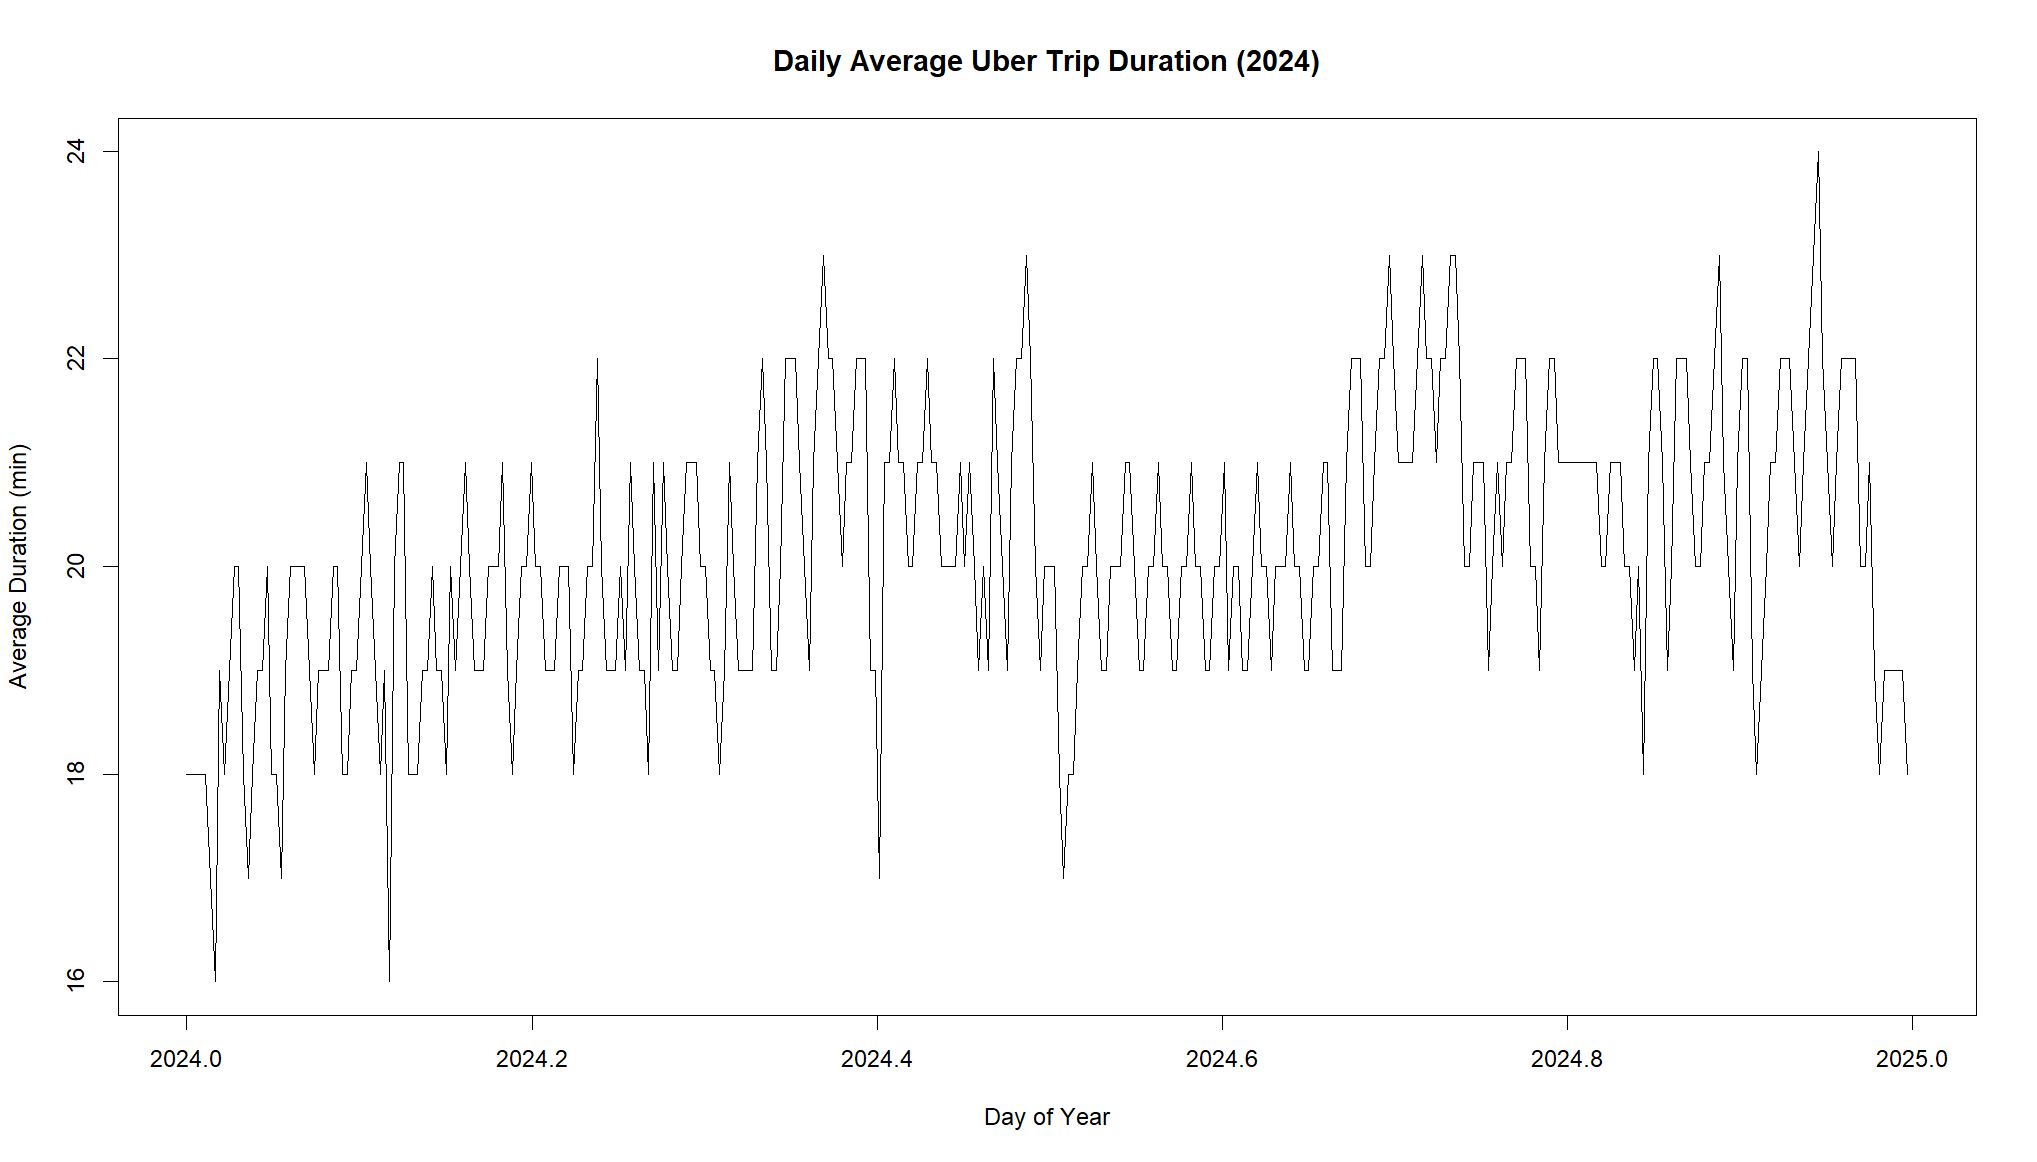
\includegraphics[width=\textwidth]{avg_trip_duration_simple.png}
  \caption{Daily average Uber trip duration in NYC for 2024.}
  \label{fig:initial_plot}
\end{figure}

\subsection{Annotated Time Series and Weekly Seasonality}
In an attempt to expose more patterns, a second version of the time series plot was created with Fridays, Saturdays, Sundays, and the major holidays in the United States highlighted (Figure~\ref{fig:timeseries_plot}, Listing ~\ref{lst:r_plot_weekend_holidays}). This annotated visualization reveals more structured weekly seasonality, with higher average durations occurring more frequently on weekends. Holidays such as Memorial Day, Independence Day, and Christmas are associated with pronounced decreases in duration.

\begin{figure}
  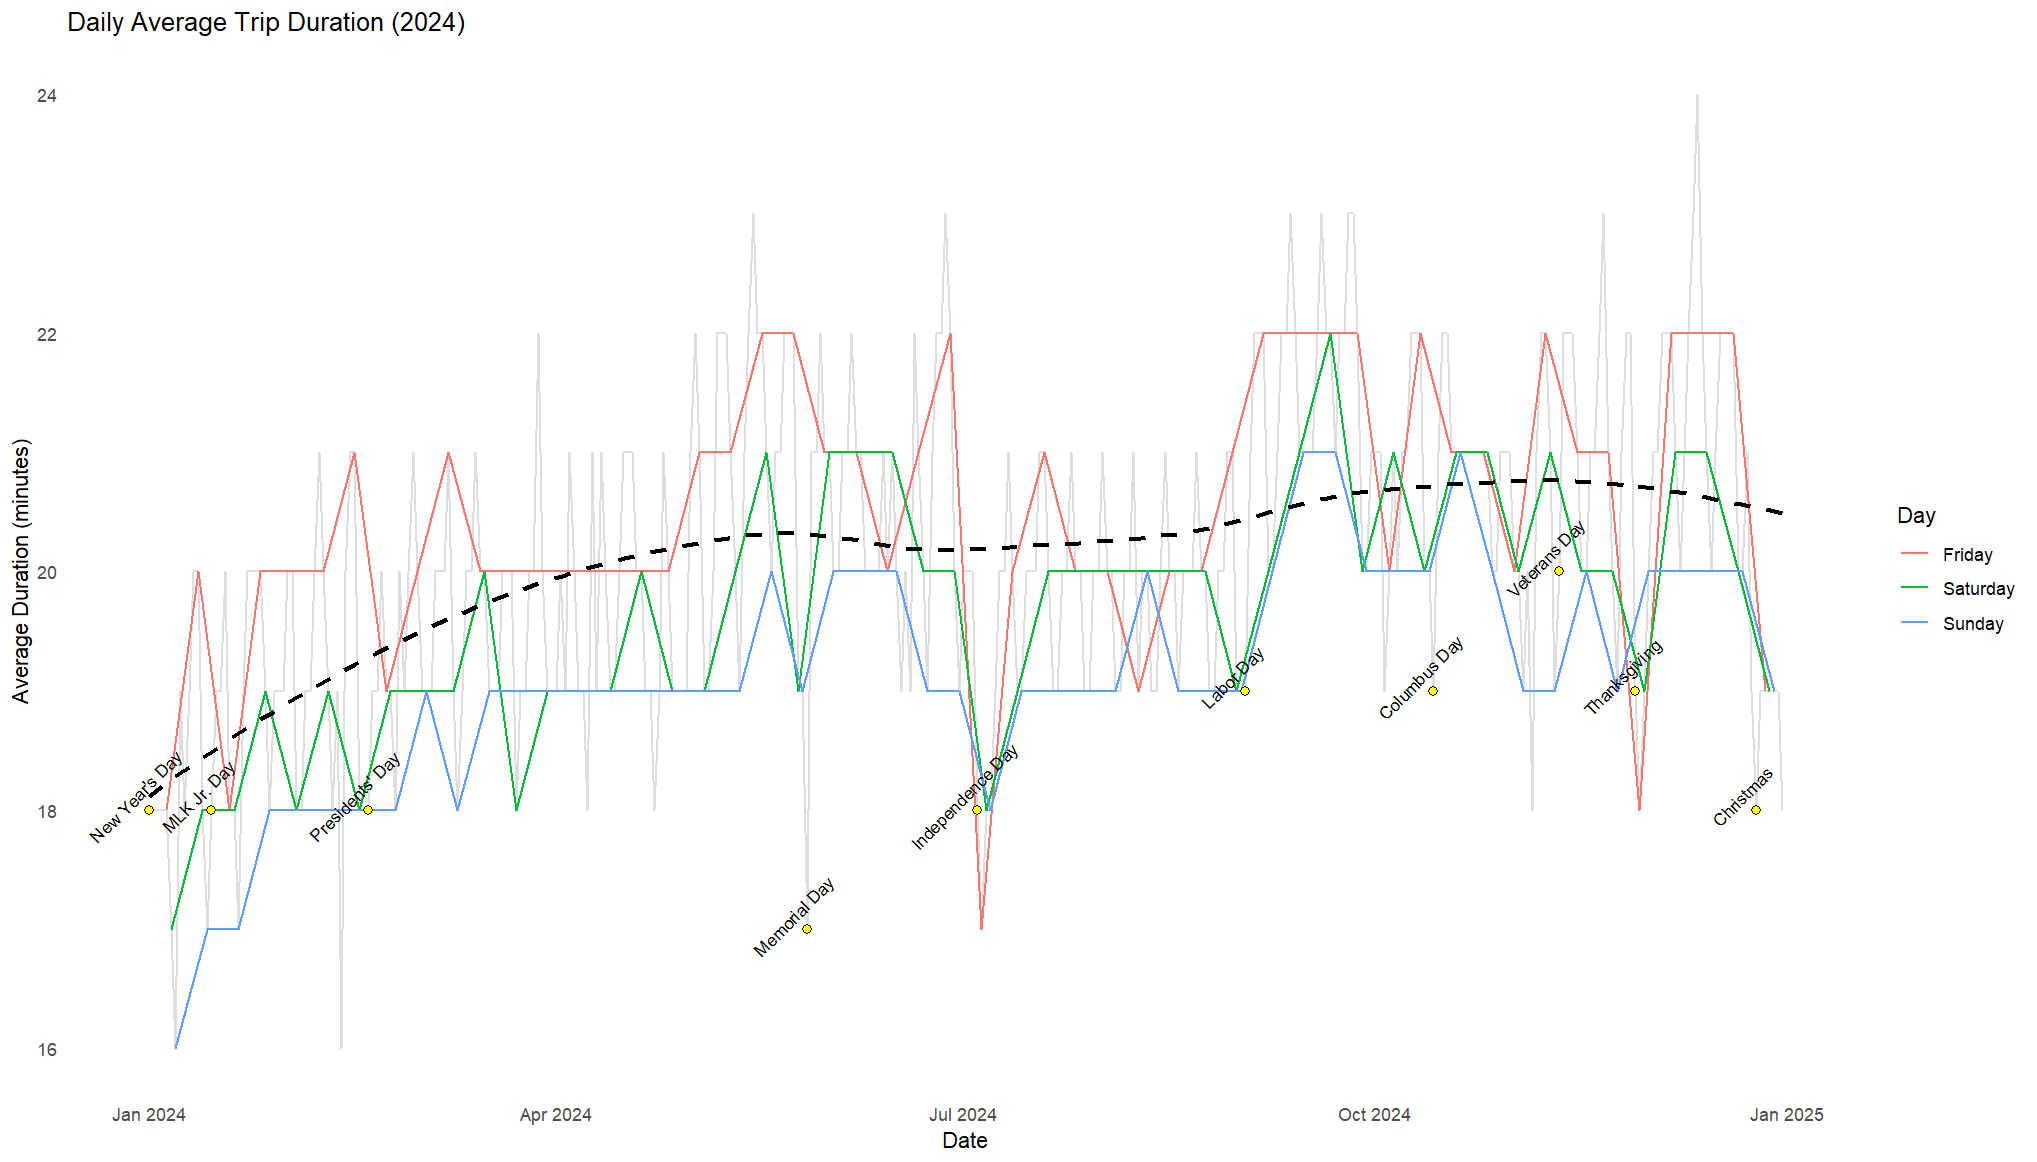
\includegraphics[width=\textwidth]{avg_trip_duration_by_day.png}
  \caption{Daily average Uber trip duration in NYC for 2024, with weekends and holidays highlighted.}
  \label{fig:timeseries_plot}
\end{figure}

\subsection{Stationarity Assessment}
To determine whether the daily average Uber trip duration series is stationary, we performed the Augmented Dickey-Fuller (ADF) test (Listing ~\ref{lst:r_adf_test}). The ADF test yielded a $p$-value of 0.04612. Because the $p$-value is less than 0.05, we reject the null hypothesis at the significance level $\alpha$=0.05. Therefore, there is statistical evidence to suggest that the time series is stationary.

\subsection{Autocorrelation and Partial Autocorrelation Analysis}
The ACF plot (Figure~\ref{fig:acf_plot}, Listing~\ref{lst:r_acf}) shows a slow and gradual decline, consistent with a non-stationary series. This pattern suggests the presence of a trend and the need to differentiate the series to induce stationarity. Significant autocorrelation at multiple lags may also indicate latent seasonality.

\begin{figure}
  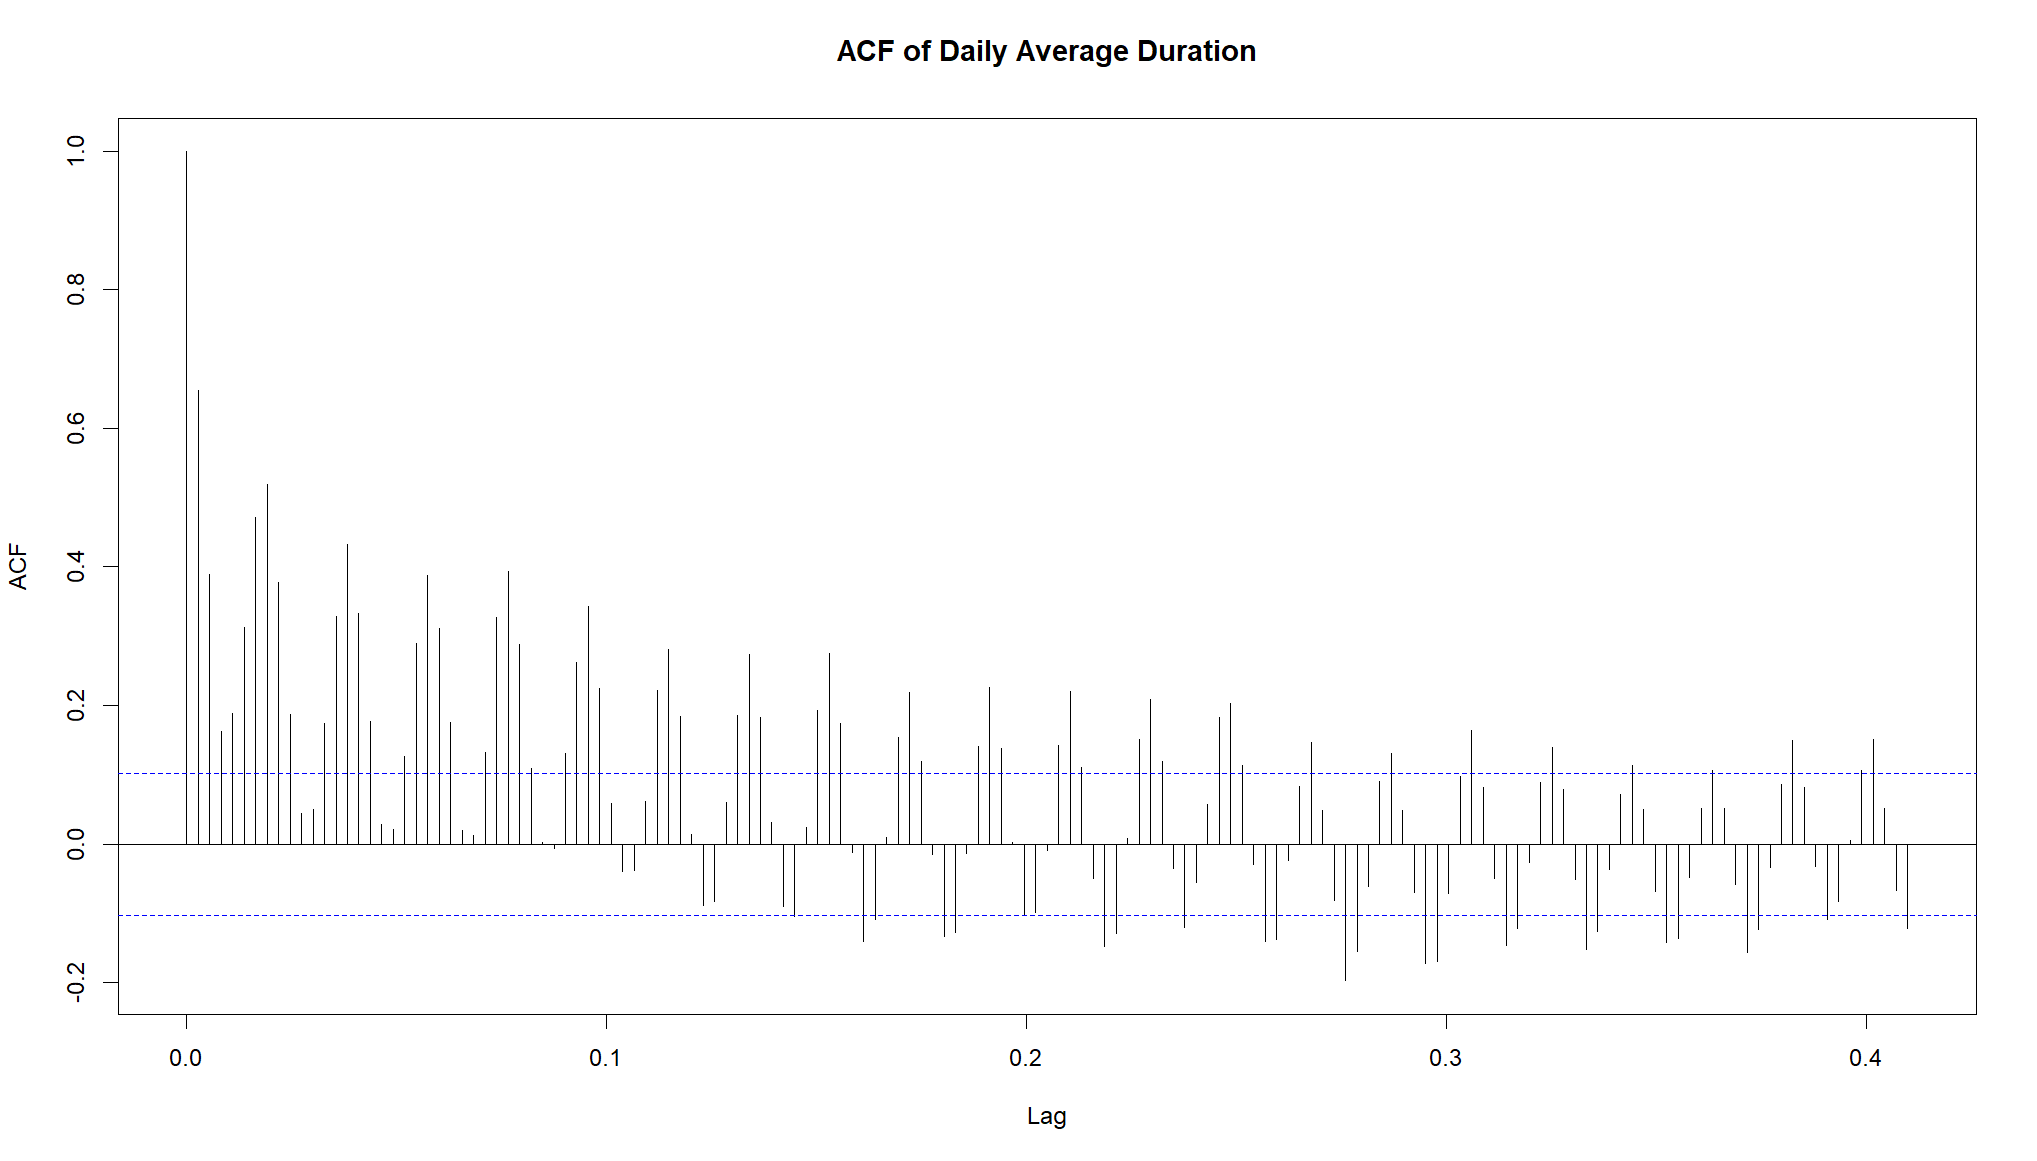
\includegraphics[width=\textwidth]{finalproject/images/acf-plot.png}
  \caption{Autocorrelation Function (ACF) plot of daily average trip durations. The plot shows a slow decay, suggesting non-stationarity and potential seasonality in the data.}
  \label{fig:acf_plot}
\end{figure}

The PACF plot (Figure~\ref{fig:pacf_plot}, Listing~\ref{lst:r_pacf}) shows a large spike at lag 1, followed by a tapering tail of smaller spikes. This pattern suggests the existence of an autoregressive (AR) structure in the series. The combination of these findings supports the consideration of ARIMA modeling, potentially with seasonal differencing.

\begin{figure}
  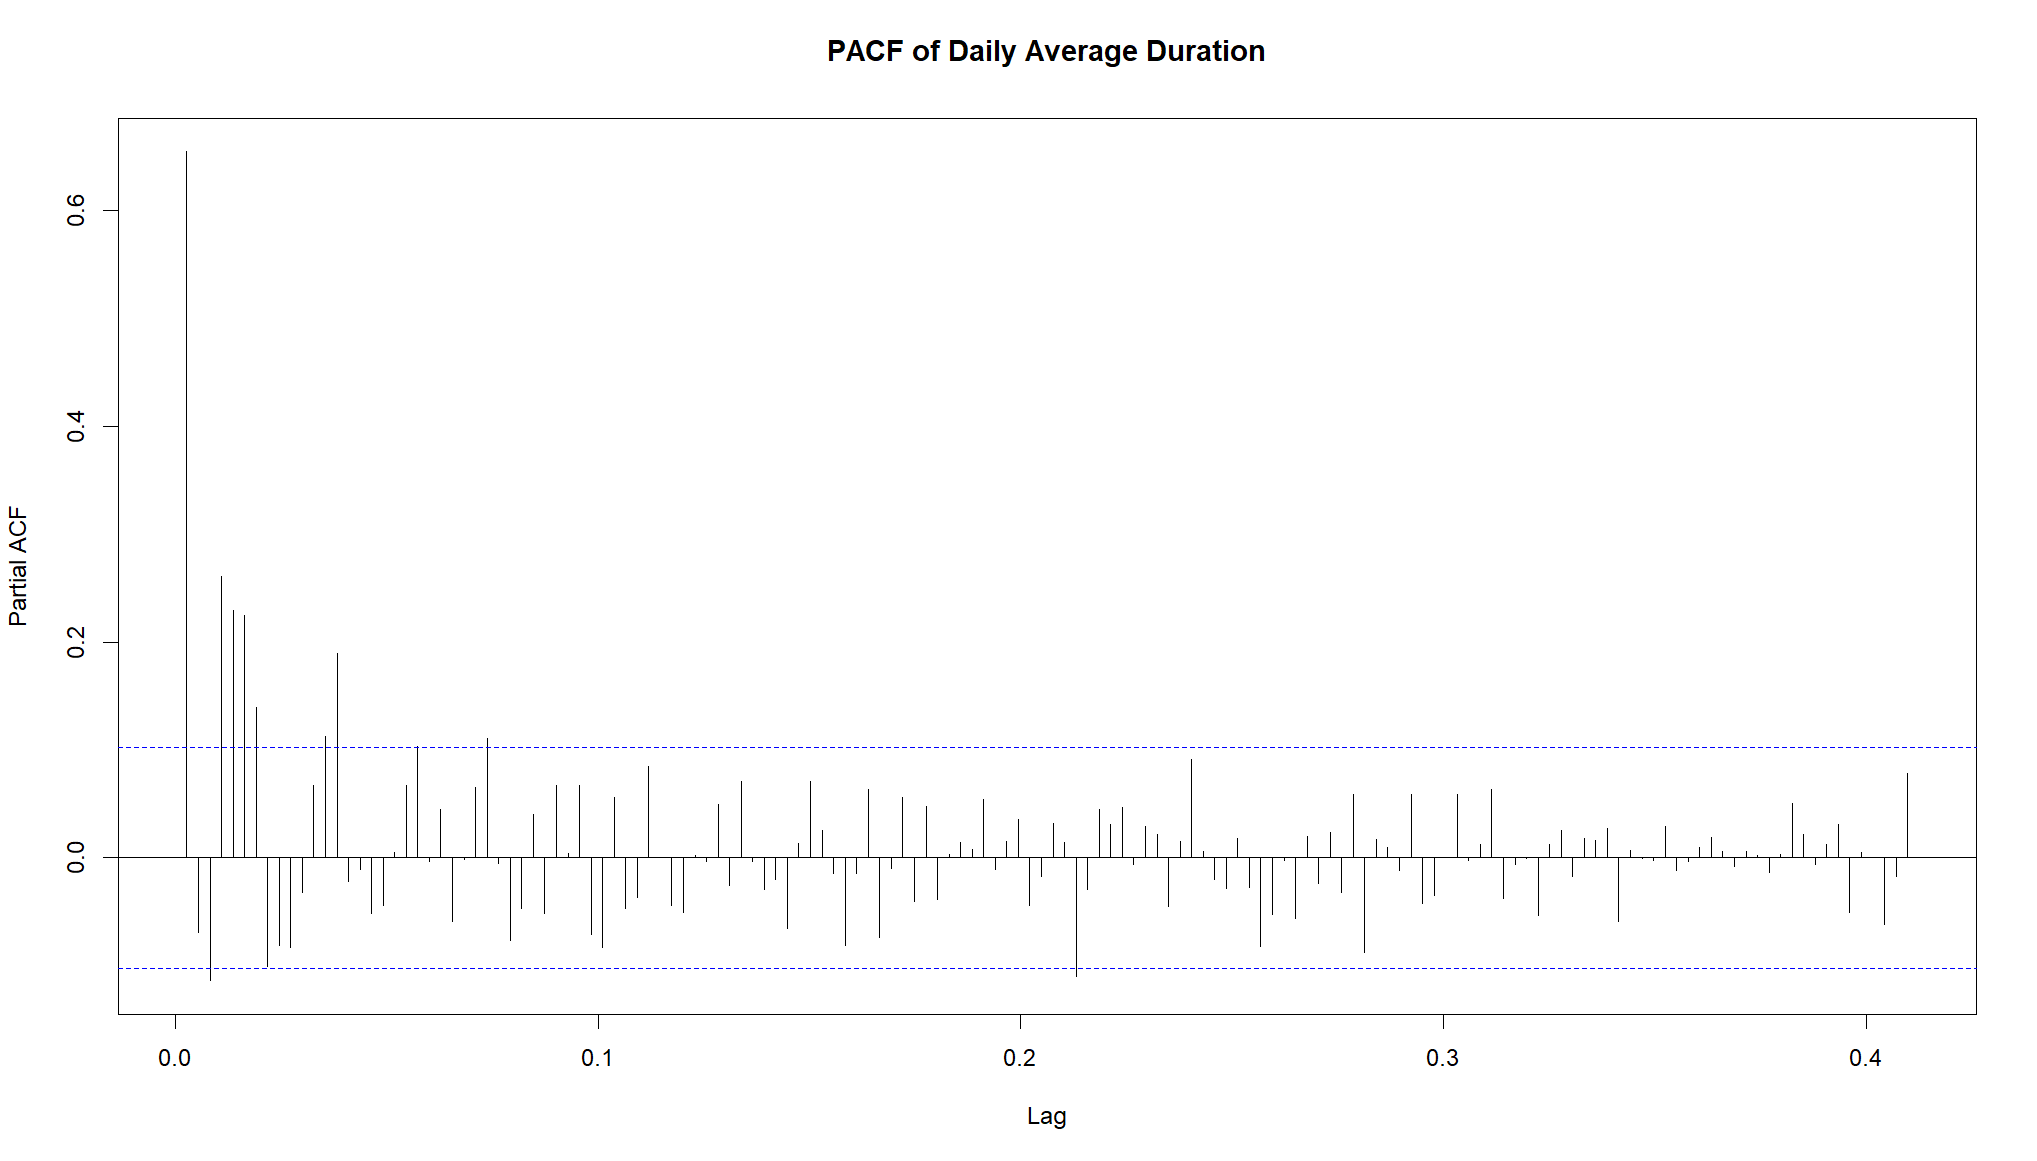
\includegraphics[width=\textwidth]{finalproject/images/pacf-plot.png}
  \caption{Partial Autocorrelation Function (PACF) plot of daily average trip durations. The sharp drop after the first few lags indicates the presence of autoregressive components.}
  \label{fig:pacf_plot}
\end{figure}

\subsection{Reconciling ADF and ACF/PACF Findings}
Although the ADF test returned a $p$-value of 0.04612, suggesting stationarity at significance level $\alpha$=0.05, the ACF and PACF plots exhibit patterns indicative of non-stationarity, including a slow decay in autocorrelation. This discrepancy implies that the series may be only marginally stationary or trend-stationary. To address this, further differencing is warranted in the model's subsequent development.


\section{Secondary Analysis and Modeling}

\subsection{Model Fitting}

To model the average daily Uber trip duration, we applied the \texttt{auto.arima()} function from the \texttt{forecast} package in R, which identified an ARIMA(3,1,2) model as the best fit (Figure \ref{fig:arima_coefficients}, Listing~\ref{lst:r_arima}).

\begin{figure}[ht]
\centering
\label{fig:arima_coefficients}
\begin{lstlisting}[basicstyle=\ttfamily]
ARIMA(3,1,2)

Coefficients:
         ar1      ar2      ar3      ma1     ma2
      0.8166  -0.4500  -0.3559  -1.2271  0.6940
\end{lstlisting}
\caption{Estimated ARIMA(3,1,2) model coefficients.}
\end{figure}

The model includes three autoregressive terms (AR) and two moving average terms (MA), with one order of differencing. The residuals from this model were analyzed using diagnostic plots and the Ljung-Box test to assess the adequacy of the model.

\begin{figure}
  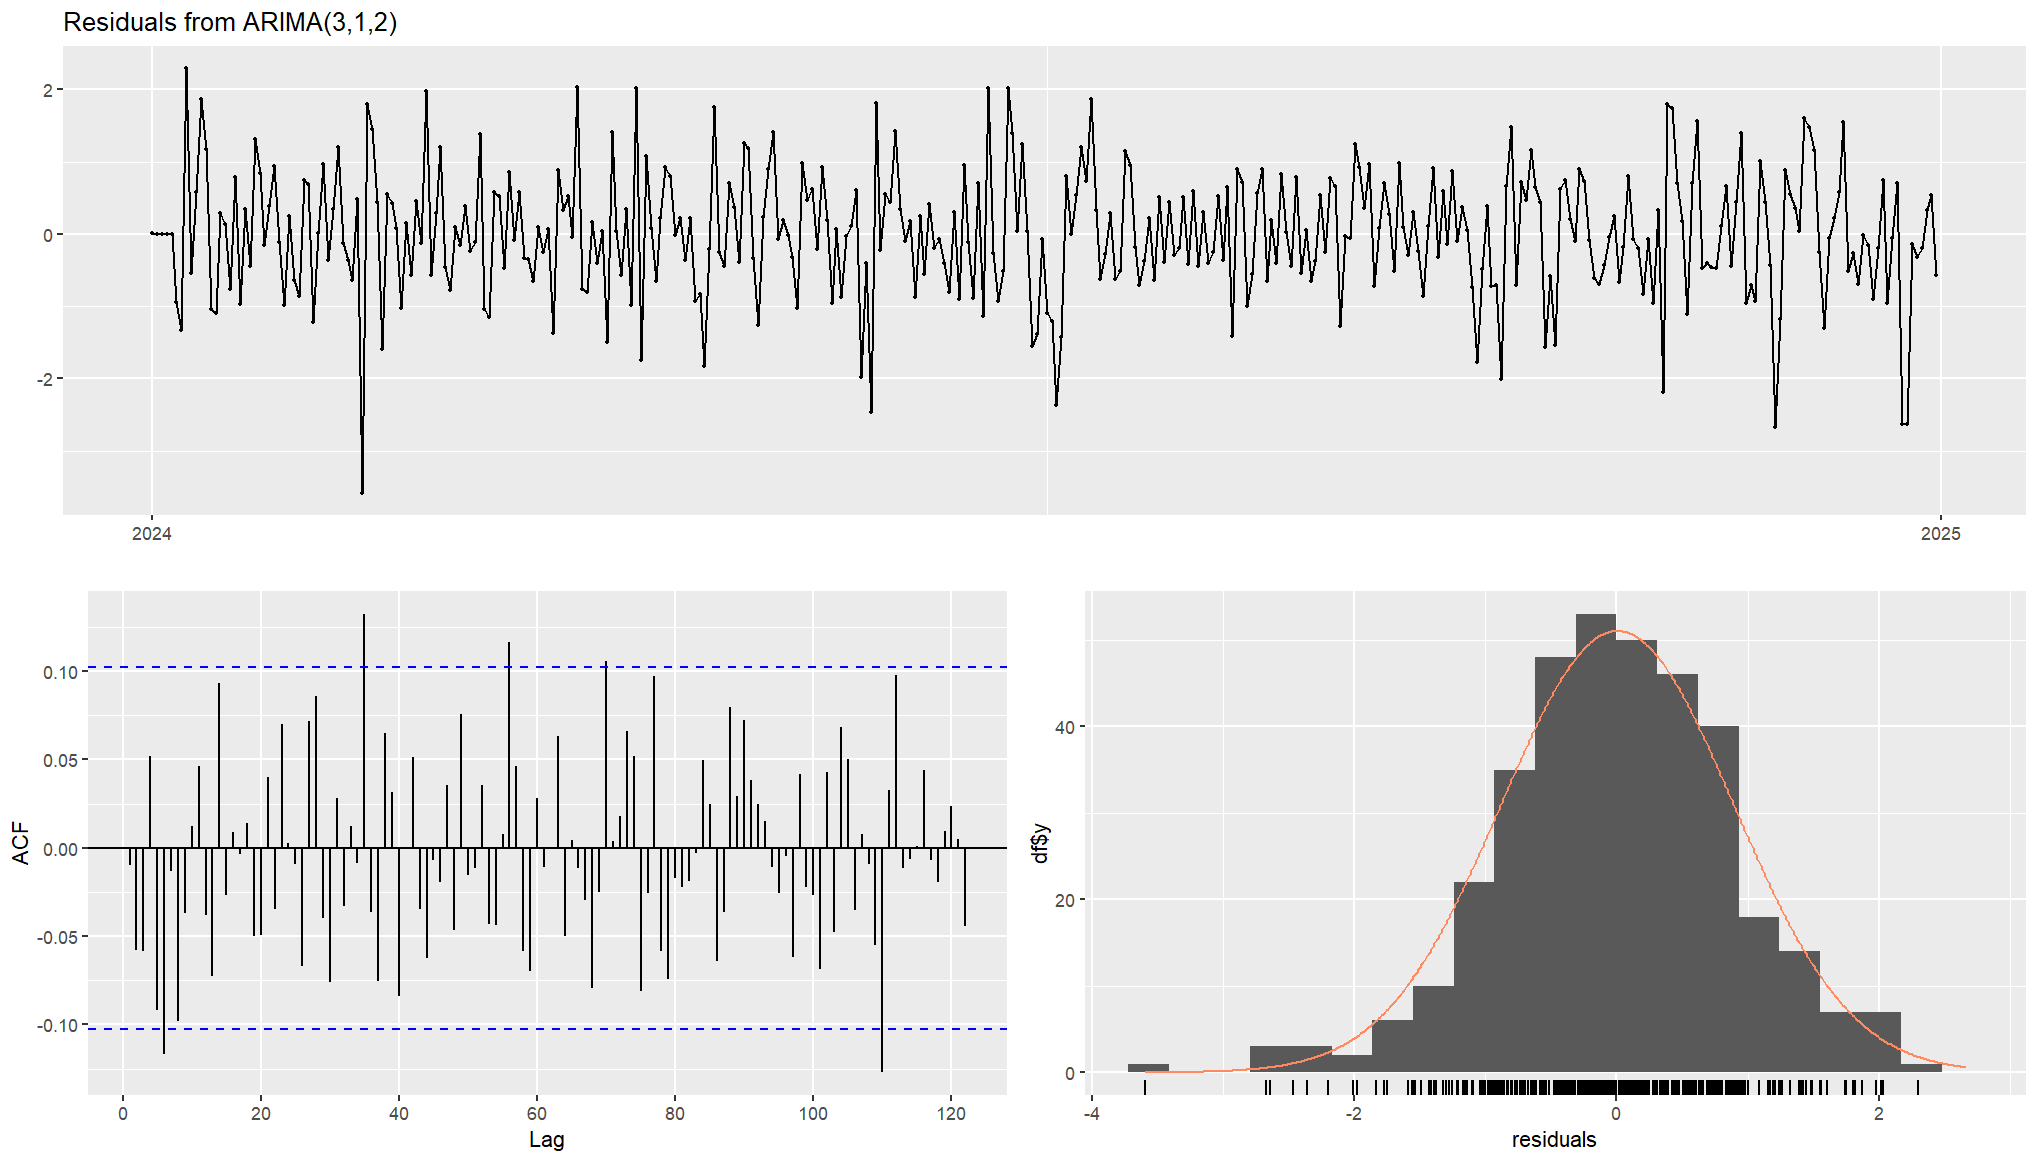
\includegraphics[width=\textwidth]{finalproject/images/arima-residuals.png}
  \caption{Residual diagnostics for ARIMA(3,1,2): time plot (top), ACF of residuals (bottom left), and histogram with normal distribution curve (bottom right).}
  \label{fig:arima_residuals}
\end{figure}

The residual plots (Figure~\ref{fig:arima_residuals}, Listing~\ref{lst:r_arima_resid}) suggest that the residuals are centered around zero with constant variance and no strong autocorrelation. The ACF plot of residuals confirms the absence of significant autocorrelation at most lags.

The Ljung-Box test (Listing~\ref{lst:r_arima_resid}) further supports the adequacy of the model ($p = 0.05184$). Since the $p$-value is slightly above 0.05, we do not reject the null hypothesis that the residuals are white noise. Therefore, a first differencing has resulted in stationarity.

\subsection{Fitted Model Equation}

The fitted ARIMA(3,1,2) model can be written as shown in Equation \ref{eq:arima_model}.

\begin{multline}
\label{eq:arima_model}
Y_t = Y_{t-1} 
+ 0.8166 (Y_{t-1} - Y_{t-2}) 
- 0.4500 (Y_{t-2} - Y_{t-3}) 
- 0.3559 (Y_{t-3} - Y_{t-4}) \\
+ \varepsilon_t 
- 1.2271 \varepsilon_{t-1} 
+ 0.6940 \varepsilon_{t-2}
\end{multline}

where \( Y_t \) denotes the average trip duration at time \( t \) and \( \varepsilon_t \) is a white noise error term.

The residual diagnostics and statistical tests provide evidence that this model is a reasonable choice for forecasting the average daily trip durations (Figure \ref{fig:arima_residuals}).

\subsection{Interpretation of the ARIMA Model}

The fitted ARIMA(3,1,2) model suggests that the average Uber trip duration on a given day is influenced by a combination of past values and past random fluctuations. 

The \textbf{autoregressive (AR)} component means that the duration is partly predicted using the trip durations of the last three days. If durations have been increasing or decreasing in recent days, this trend is likely to continue in the short term. 

The \textbf{integrated (I)} component—represented by the differencing step - accounts for nonstationarity, helping the model focus on changes from one day to the next rather than absolute levels.

The \textbf{moving average (MA)} component adjusts the predictions based on the last two prediction errors. For example, if a previous day's duration was unusually high or low due to unexpected traffic or a weather event, the MA terms help correct for that anomaly in future predictions.

Together, these components allow the ARIMA model to capture both consistent temporal patterns and unexpected variations in ride durations, making it a practical tool to forecast and understand urban mobility trends over time.


\subsection{Forecasting}

To evaluate the predictive utility of the fitted model, we generated a 14-day forecast using the ARIMA(3,1,2) model (Listing~\ref{lst:r_forecast}). Figure~\ref{fig:forecast_plot} shows the projected average trip duration along with the 80\% and 95\% confidence intervals (Listing~\ref{lst:r_forecast_plot}).

\begin{figure}
  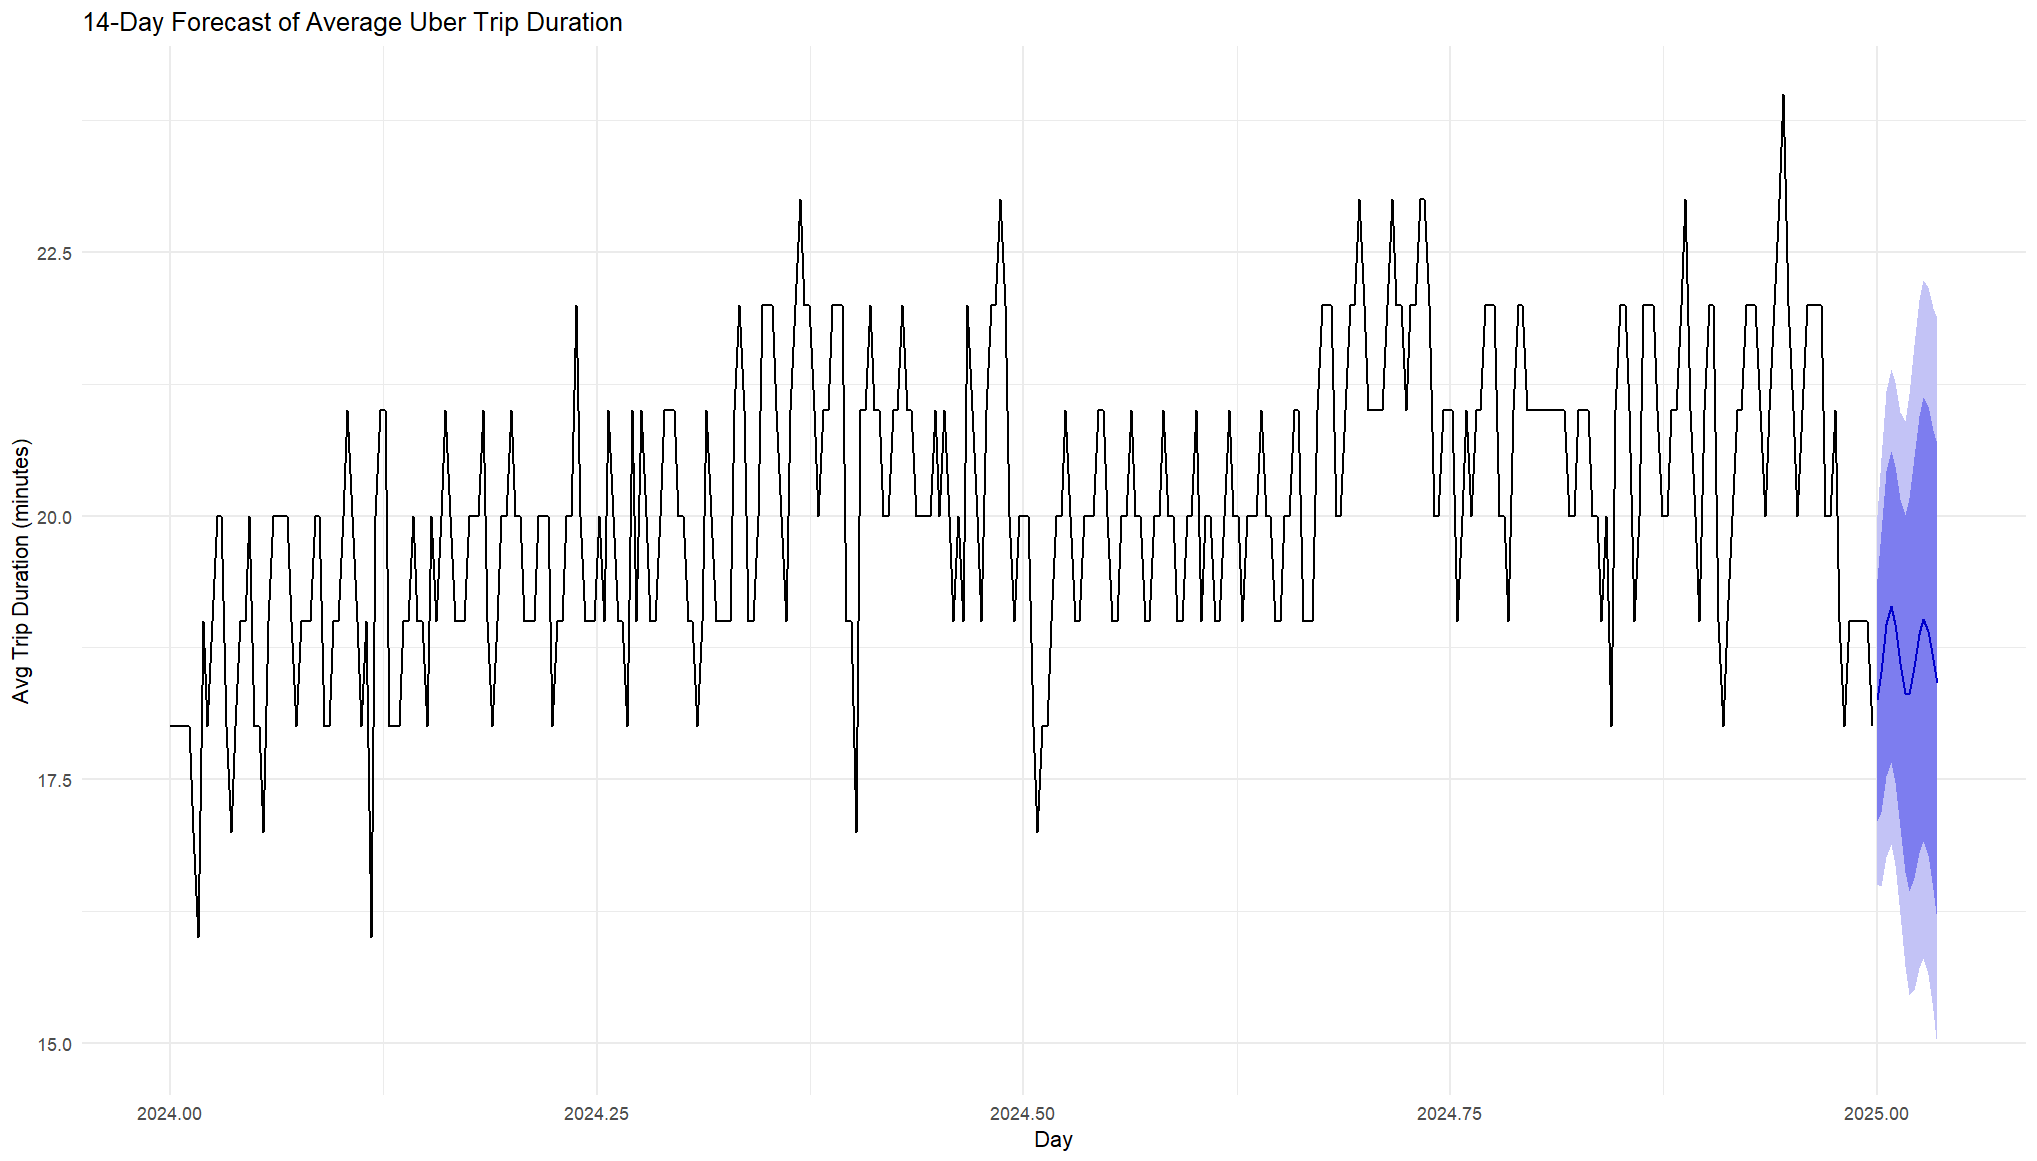
\includegraphics[width=\textwidth]{finalproject/images/forecast-plot.png}
  \caption{14-day forecast of average Uber trip duration with 80\% and 95\% confidence intervals.}
  \label{fig:forecast_plot}
\end{figure}

The forecast suggests that the average travel duration is expected to stabilize in the range of 18 to 19 minutes. Although point forecasts are relatively flat, the widening confidence intervals reflect increased uncertainty over time. The forecasted values for the next 14 days, along with their 80\% and 95\% prediction intervals (Listing~\ref{lst:r_forecast_table}), are shown in Table~\ref{tab:forecast_values}.

\begin{table}[ht]
\centering
\caption{14-day forecast of average trip durations with 80\% and 95\% prediction intervals.}
\label{tab:forecast_values}
\begin{tabular}{lrrrrr}
\toprule
Date & Forecast & Lo 80 & Hi 80 & Lo 95 & Hi 95 \\
\midrule
2025-01-01 & 18.25 & 17.11 & 19.40 & 16.50 & 20.00 \\
2025-01-02 & 18.52 & 17.19 & 19.85 & 16.48 & 20.55 \\
2025-01-03 & 18.98 & 17.53 & 20.42 & 16.76 & 21.19 \\
2025-01-04 & 19.14 & 17.67 & 20.62 & 16.89 & 21.40 \\
2025-01-05 & 18.98 & 17.48 & 20.48 & 16.68 & 21.27 \\
2025-01-06 & 18.60 & 17.04 & 20.16 & 16.22 & 20.99 \\
2025-01-07 & 18.31 & 16.62 & 20.00 & 15.73 & 20.90 \\
2025-01-08 & 18.30 & 16.44 & 20.17 & 15.46 & 21.15 \\
2025-01-09 & 18.56 & 16.56 & 20.56 & 15.50 & 21.62 \\
2025-01-10 & 18.88 & 16.80 & 20.95 & 15.71 & 22.04 \\
2025-01-11 & 19.02 & 16.92 & 21.13 & 15.80 & 22.24 \\
2025-01-12 & 18.91 & 16.78 & 21.04 & 15.65 & 22.17 \\
2025-01-13 & 18.64 & 16.46 & 20.81 & 15.31 & 21.97 \\
2025-01-14 & 18.42 & 16.15 & 20.68 & 14.95 & 21.88 \\
\bottomrule
\end{tabular}
\end{table}

Residual diagnostics (Figure~\ref{fig:forecast_diagnostics}, Listing~\ref{lst:r_forecast_resid}) indicate that residuals are approximately normally distributed and do not exhibit significant autocorrelation, as confirmed by the Ljung-Box test ($p = 0.0518$), suggesting that the model adequately captures the structure in the data.

\begin{figure}
  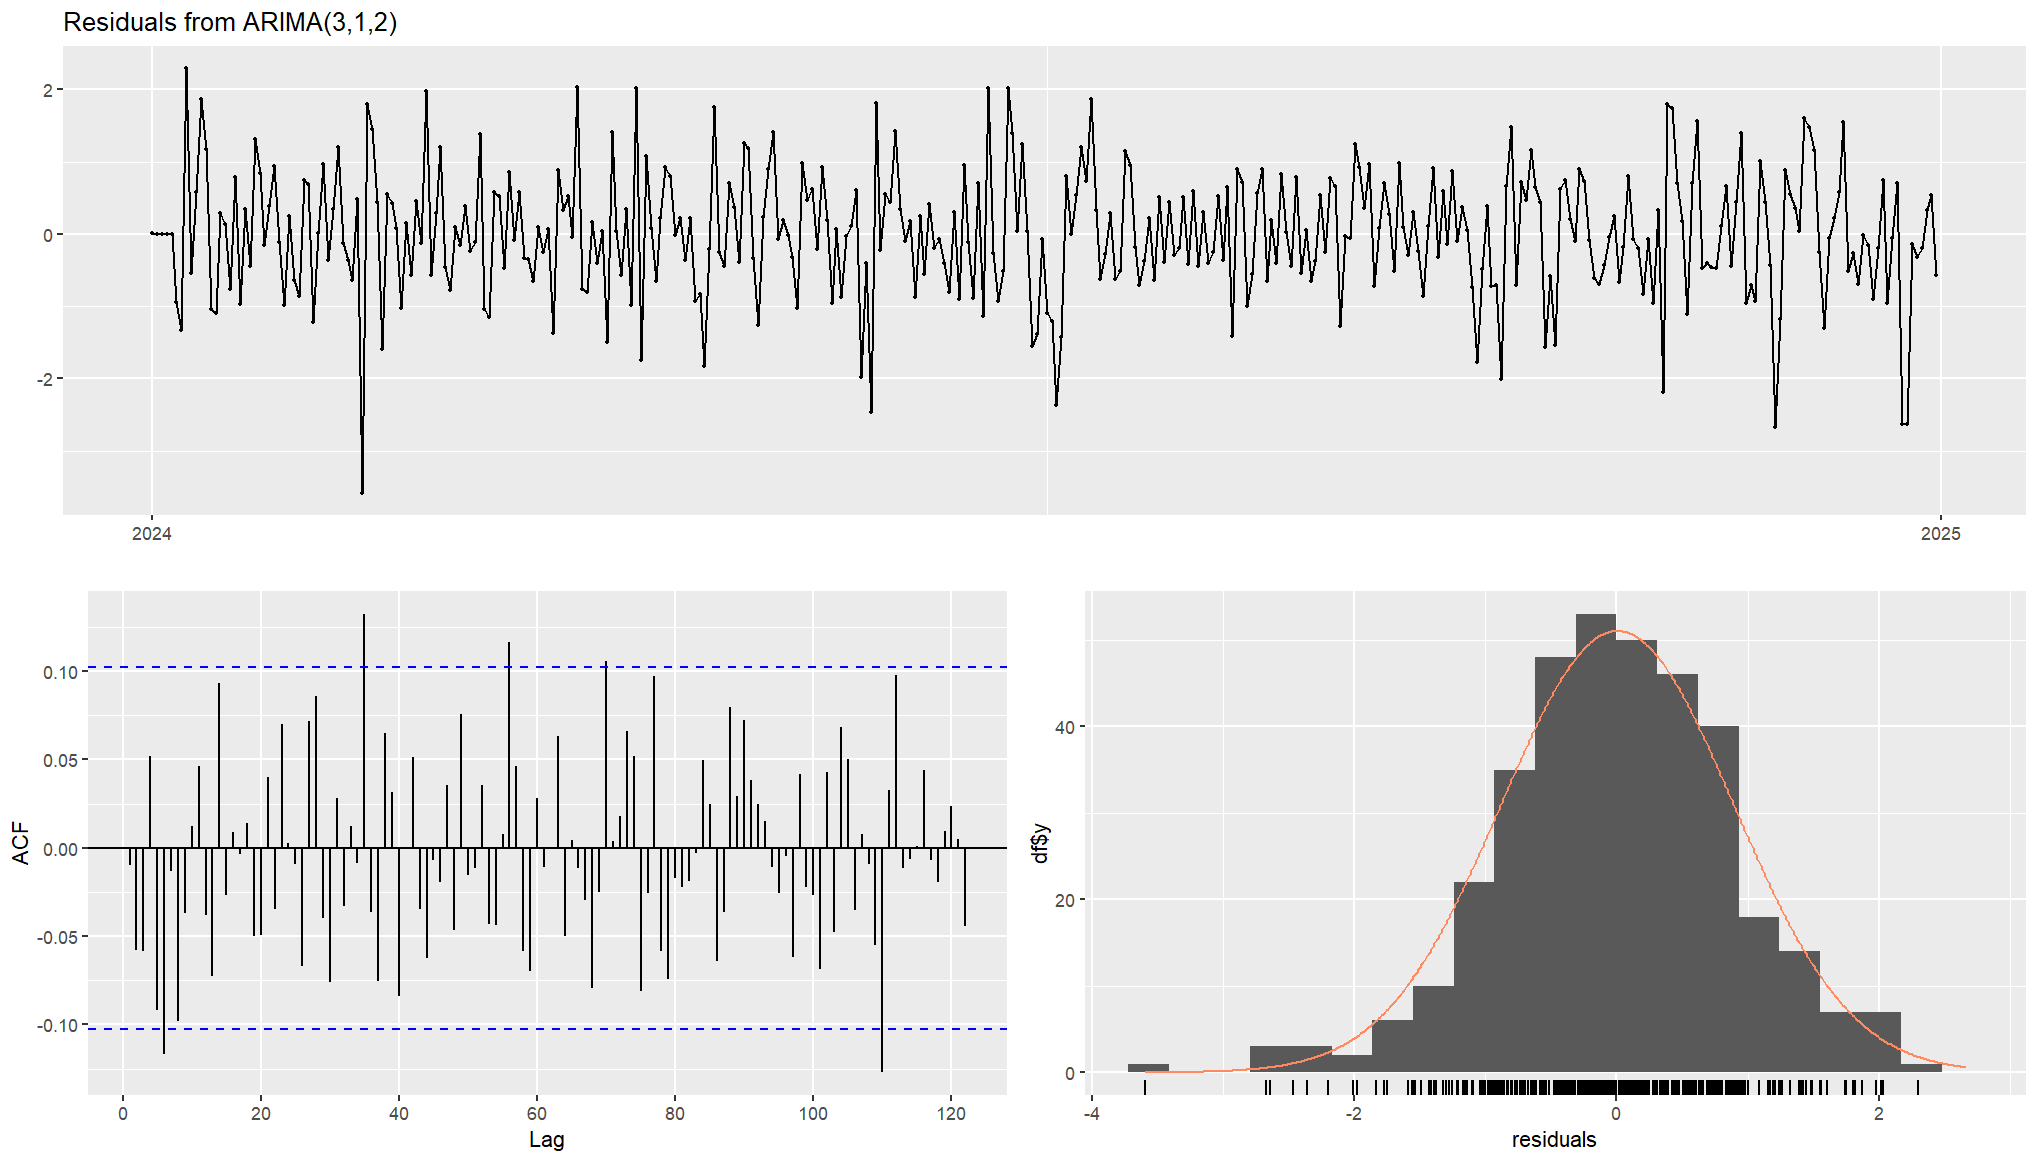
\includegraphics[width=\textwidth]{finalproject/images/forecast-residuals.png}
  \caption{Residual diagnostics for the 14-day ARIMA forecast: time plot (top), ACF of residuals (bottom left), and histogram with normal distribution curve (bottom right). }
  \label{fig:forecast_diagnostics}
\end{figure}


\section{Discussion and Conclusion}

This project set out to analyze temporal trends in Uber trip durations using New York City's High-Volume For-Hire Vehicle (FHV) dataset for 2024. The analysis focused on daily average trip durations and applied time series modeling techniques to identify patterns and forecast future behavior.

The ARIMA(3,1,2) model fitted to the data demonstrated a reasonably good fit, with low residual autocorrelation and a Ljung-Box test $p$-value close to the significance threshold. The model successfully captured temporal dynamics and was informed by stationarity checks, ACF, and PACF analysis. The results indicate that the duration of Uber rides exhibits regular fluctuations, with weekends and most holidays showing elevated travel times, likely due to increased congestion or changes in demand patterns.

The fitted ARIMA model was also used to generate a 14-day forecast of average trip durations. The forecast suggests continued fluctuations with point predictions that ranged from approximately 18 to 19 minutes. The 95\% prediction intervals provide a reasonable range of uncertainty, with the lower bounds staying above 16 minutes and the upper bounds exceeding 21 minutes at times. This demonstrates the model's utility for short-term forecasting of ride duration trends.

Importantly, the structure of the ARIMA model provides interpretable insights. The autoregressive (AR) terms reflect the persistence of duration trends over three days, while the moving average (MA) terms capture the impact of recent anomalies such as sudden spikes or drops in trip duration due to unpredictable events such as traffic disruptions or weather. The presence of two MA terms allows the model to learn from forecasting errors over the past two days, making the forecasts more adaptive and robust to short-term volatility.

One strength of the analysis was the use of big data tools (PySpark) to preprocess more than 200 million records into a manageable time series format. This preprocessing enabled meaningful aggregation and reduced the computational burden on R, which was used for modeling and visualization. Visualizing holidays and weekends also helped contextualize anomalies and recurring patterns in the data.

However, the study has several limitations. The univariate ARIMA model focuses solely on past values and past errors in average trip duration, without explicitly incorporating external variables such as weather conditions, traffic incidents, or special events. Although moving average terms help absorb recent unexplained anomalies, they do not directly account for known external factors that could improve predictive accuracy. Additionally, aggregating data at the daily level smooths over intraday variations, potentially obscuring important temporal dynamics. Finally, the dataset includes only Uber trips, which may limit the generalization of the findings to the broader transportation or ride-hailing ecosystem.

Future work could include incorporating a multivariate approach to examine the relationships between trip duration, trip count, and distance. More granular models (for example, hourly data) or spatial analysis could also reveal deeper insights into congestion dynamics across neighborhoods.

In conclusion, this project demonstrates the feasibility and value of using large-scale ride-hailing data for time-series analysis. The findings support the use of predictive models to anticipate congestion trends and could inform urban planning, fleet management, or dynamic pricing strategies.


\appendix

\section{R Time Series Modeling and Visualization Code}
\label{appendix:rcode}
\begin{lstlisting}[style=rstyle, caption={Loading and Plotting Time Series}, label={lst:r_ts_plot}]

library(ggplot2)

data <- read.csv(file.path(getwd(), "../data", "fhvhv_tripdata_2024_uber_timeseries.csv"))
ts_data <- ts(data$avg_duration_min, frequency = 366, start = c(2024, 1))

plot(ts_data,
     main = "Daily Average Uber Trip Duration (2024)",
     xlab = "Day of Year",
     ylab = "Average Duration (min)")
\end{lstlisting}


\begin{lstlisting}[style=rstyle, caption={Plot Highlighting Weekends and Holidays}, label={lst:r_plot_weekend_holidays}]

library(dplyr)

data$pickup_date <- as.Date(data$pickup_date)

data <- data %>%
  mutate(weekday = weekdays(pickup_date))

fridays <- filter(data, weekday == "Friday")
saturdays <- filter(data, weekday == "Saturday")
sundays <- filter(data, weekday == "Sunday")

holidays <- data.frame(
  date = as.Date(c(
    "2024-01-01",  # New Year's Day
    "2024-01-15",  # Martin Luther King Jr. Day
    "2024-02-19",  # Presidents' Day
    "2024-05-27",  # Memorial Day
    "2024-07-04",  # Independence Day
    "2024-09-02",  # Labor Day
    "2024-10-14",  # Columbus Day
    "2024-11-11",  # Veterans Day
    "2024-11-28",  # Thanksgiving
    "2024-12-25"   # Christmas
  )),
  label = c(
    "New Year's Day", "MLK Jr. Day", "Presidents' Day", "Memorial Day", "Independence Day",
    "Labor Day", "Columbus Day", "Veterans Day", "Thanksgiving", "Christmas"
  )
)

holidays$avg_duration_min <- data$avg_duration_min[match(holidays$date, data$pickup_date)]

ggplot(data, aes(x = pickup_date, y = avg_duration_min)) +
  geom_line(color = "gray", alpha = 0.5) +
  geom_line(data = fridays, aes(color = "Friday")) +
  geom_line(data = saturdays, aes(color = "Saturday")) +
  geom_line(data = sundays, aes(color = "Sunday")) +
  geom_point(data = holidays, aes(x = date, y = avg_duration_min), 
             color = "black", fill = "yellow", size = 2, shape = 21) +
  geom_text(data = holidays, aes(x = date, y = avg_duration_min, label = label), 
            vjust = -1, size = 3, angle = 45) +
  scale_color_manual(
    values = c(
      "Friday" = "#332288", 
      "Saturday" = "#EE7733",
      "Sunday" = "#117733"   
    )
  ) +
  labs(
    title = "Daily Average Trip Duration (2024)",
    x = "Date", y = "Average Duration (minutes)",
    color = "Day"
  ) +
  theme_minimal() +
  theme(
    panel.grid.major = element_blank(),
    panel.grid.minor = element_blank()
  )

\end{lstlisting}

\begin{lstlisting}[style=rstyle, caption={ Augmented Dickey-Fuller (ADF) Test}, label={lst:r_adf_test}]
library(tseries)
adf.test(ts_data)
\end{lstlisting}

\begin{lstlisting}[style=rstyle, caption={ ACF Plot}, label={lst:r_acf}]
acf(ts_data, main = "ACF of Daily Average Duration", lag.max = 150)
\end{lstlisting}

\begin{lstlisting}[style=rstyle, caption={ PACF Plot}, label={lst:r_pacf}]
pacf(ts_data, main = "PACF of Daily Average Duration", lag.max = 150)
\end{lstlisting}

\begin{lstlisting}[style=rstyle, caption={ ARIMA Model}, label={lst:r_arima}]
library(forecast)
diff_data <- diff(ts_data)
fit <- auto.arima(ts_data)
summary(fit)
\end{lstlisting}

\begin{lstlisting}[style=rstyle, caption={ ARIMA Model Residual Plots}, label={lst:r_arima_resid}]
checkresiduals(fit)
\end{lstlisting}

\begin{lstlisting}[style=rstyle, caption={ 14-day Forecast}, label={lst:r_forecast}]
h <- 14
forecast_result <- forecast(fit, h = h)
\end{lstlisting}

\begin{lstlisting}[style=rstyle, caption={ Plot of 14-day Forecast}, label={lst:r_forecast_plot}]
autoplot(forecast_result) +
  labs(
    title = "14-Day Forecast of Average Uber Trip Duration",
    x = "Day",
    y = "Avg Trip Duration (minutes)"
  ) +
  theme_minimal()
\end{lstlisting}

\begin{lstlisting}[style=rstyle, caption={ 14-day Forecast Residuals}, label={lst:r_forecast_resid}]
checkresiduals(forecast_result)
\end{lstlisting}

\begin{lstlisting}[style=rstyle, caption={ Table of Forecasted Values}, label={lst:r_forecast_table}]
start_date <- as.Date("2025-01-01")
forecast_dates <- seq.Date(from = start_date, by = "day", length.out = h)
forecast_summary <- as.data.frame(forecast_result)
formatted_forecast <- cbind(Date = forecast_dates, forecast_summary)

formatted_forecast <- within(formatted_forecast, {
  `Point Forecast` <- round(`Point Forecast`, 2)
  `Lo 80` <- round(`Lo 80`, 2)
  `Hi 80` <- round(`Hi 80`, 2)
  `Lo 95` <- round(`Lo 95`, 2)
  `Hi 95` <- round(`Hi 95`, 2)
})

print(formatted_forecast)
\end{lstlisting}

\section{PySpark Preprocessing Code}
\label{appendix:pyspark}

The following PySpark script was used to preprocess over 200 million records from the NYC FHV dataset and compute the average daily trip durations.

First, the parquet file is loaded (Listing ~\ref{lst:pyspark_load}).

\begin{lstlisting}[style=pystyle, caption={Loading FHV Data from Parquet Files}, label={lst:pyspark_load}]
!pip install pyspark
from pyspark.sql import SparkSession
from pyspark.sql.functions import col, when, to_date, avg, round

spark = SparkSession.builder.master("local[*]").appName("FHV-ts-project").getOrCreate()

data_directory = "/content/drive/MyDrive/datasets/nyc-taxi/"
df = spark.read.format("parquet").option("recursiveFileLookup", "true").load(data_directory)

\end{lstlisting}

Derived columns are added for the duration of the trip in minutes and the average speed (Listing ~\ref{lst:pyspark_derived_cols}).

\begin{lstlisting}[style=pystyle, caption={Deriving Trip Duration and Average Speed Columns}, label={lst:pyspark_derived_cols}]

df = df.withColumn("trip_duration_min", col("trip_time") / 60)
df = df.withColumn("avg_speed_mph", (col("trip_miles") / (col("trip_time") / 3600)))

\end{lstlisting}

The data is then cleaned (Listing ~\ref{lst:pyspark_cleaning}):
\begin{itemize}
    \item Trips with zero or negative trip durations are removed.
    \item Outliers are removed: \begin{itemize}
        \item Trips longer than 2 hours and shorter than 1 minute.
        \item Trips longer than 100 miles and less than 0.1 miles.
        \item Average speed of greater than 80 mph and less than 1 mph.
    \end{itemize}
    
\end{itemize}

\begin{lstlisting}[style=pystyle, caption={Data cleaning code}, label={lst:pyspark_cleaning}]

df_clean = df.filter(
    (col("trip_duration_min") > 0) &
    (col("trip_miles") > 0) &
    (col("avg_speed_mph") > 0)
)

df_clean = df_clean.filter(
    (col("trip_duration_min") <= 120) &
    (col("trip_duration_min") >= 1) &
    (col("trip_miles") <= 100) &
    (col("trip_miles") >= 0.1) &
    (col("avg_speed_mph") <= 80) &
    (col("avg_speed_mph") >= 1)
)
\end{lstlisting}

The outliers are then removed (Listing ~\ref{lst:pyspark_outliers}).

\begin{lstlisting}[style=pystyle, caption={Removing outliers code}, label={lst:pyspark_outliers}]

columns_to_check = ["trip_duration_min", "trip_miles", "avg_speed_mph"]
iqr_dict = {}

for col_name in columns_to_check:
    q1, q3 = df_clean.approxQuantile(col_name, [0.25, 0.75], 0.01)
    iqr = q3 - q1
    iqr_dict[col_name] = (q1, q3, iqr)
    print(f"IQR for {col_name}: {iqr_dict[col_name][2]}")
    print(f"  Q1 for {col_name}: {iqr_dict[col_name][0]}")
    print(f"  Q3 for {col_name}: {iqr_dict[col_name][1]}")

iqr_duration = iqr_dict["trip_duration_min"][2]
iqr_miles = iqr_dict["trip_miles"][2]
iqr_speed = iqr_dict["avg_speed_mph"][2]

iqr_factor = 1.5

iqr_duration_15 = iqr_factor * iqr_duration
iqr_miles_15 = iqr_factor * iqr_miles
iqr_speed_15 = iqr_factor * iqr_speed

duration_upper = iqr_dict["trip_duration_min"][1] + iqr_duration_15
miles_upper = iqr_dict["trip_miles"][1] + iqr_miles_15
speed_upper = iqr_dict["avg_speed_mph"][1] + iqr_speed_15

df_final = df_clean.filter(
    (col("trip_duration_min") <= duration_upper) &
    (col("trip_miles") <= miles_upper) &
    (col("avg_speed_mph") <= speed_upper)
)
)
\end{lstlisting}

Keep only Uber trips (Listing ~\ref{lst:pyspark_uber}).

\begin{lstlisting}[style=pystyle, caption={Filter to Uber trips code}, label={lst:pyspark_uber}]
df_uber = df.filter(df["hvfhs_license_num"] == "HV0003")
\end{lstlisting}

Then the average trip duration per day is calculated (Listing ~\ref{lst:pyspark_avg_duration}).

\begin{lstlisting}[style=pystyle, caption={Calculate average daily duration code}, label={lst:pyspark_avg_duration}]

df_uber = df_uber.withColumn("pickup_date", to_date(col("pickup_datetime")))

df_daily_avg = df_uber.groupBy("pickup_date") \
                   .agg(avg("trip_duration_min").alias("avg_duration_min")) \
                   .orderBy("pickup_date")

df_daily_avg = df_daily_avg.withColumn("avg_duration_min", round("avg_duration_min"))

\end{lstlisting}

Finally, the cleaned time series dataset is saved in a CSV file (Listing ~\ref{lst:pyspark_csv}). The resulting CSV file contains two columns - the pickup date and average trip duration for that day.

\begin{lstlisting}[style=pystyle, caption={Saving time series data code}, label={lst:pyspark_csv}]

final_path = "/content/drive/MyDrive/datasets/fhvhv_tripdata_2024_uber_timeseries.csv"

df_daily_avg.select("pickup_date", "avg_duration_min") \
         .coalesce(1) \
         .write.option("header", True) \
         .csv(final_path)

\end{lstlisting}





\bibliographystyle{plain}
\bibliography{finalproject/docs/refs}

\end{document}
